\section{Korrelationen zwischen Städten und ihrem Umland}
In \autoref{fig:highest_selected_counties} sind die Korrelationswerte zwischen den in  \autoref{sec:selected_counties} beschriebenen Städten und den zugehörigen Landkreisen für eine zeitliche Verschiebung zwischen $\tau=-50$ und $\tau=50$ als Kurven dargestellt.

Die Kurven, deren Maximum rechts der null ist, sind rot eingefärbt. Die Kurven mit dem höchsten Punkt links der null sind blau gefärbt. Die restlichen Kurven, welche am für $\tau=0$ maximal werden, sind grün gefärbt.
\begin{figure}[H]
    \centering
    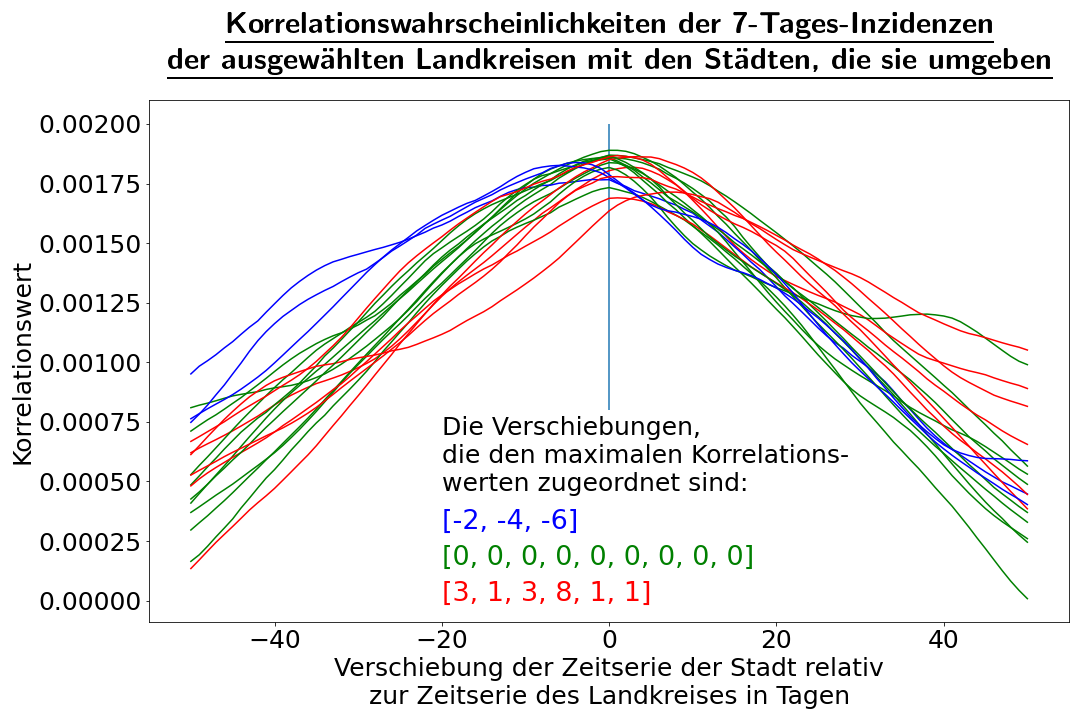
\includegraphics[width = 0.95\textwidth]{figures/Ergebnisse/highest_selected_counties.png}
    \caption{Die Korrelationswerte der 7-Tages Inzidenzen der ausgewählten Landkreise mit den Städten, die sie umgeben. Die Kurven sind je nach dem x-Wert ihres Maximums eingefärbt: Rot bei positiven x-Werten, Blau bei negativen und grün bei einem x-Wert von null.}
    \label{fig:highest_selected_counties}
\end{figure}

In dieser sehr kleinen Teilmenge weisen 50~\% der Korrelationen den höchsten Korrelationswert bei einer Verschiebung von $\tau = 0$ auf.
Bei den Korrelationen aller deutschen Landkreise untereinander liegt bei 8,7~\% der höchste Korrelationswert bei einer Verschiebung von $\tau= 0$ (8,5~\% wenn man die Korrelationen der Landkreise mit sich selbst herausrechnet).

\autoref{fig:sum_selected_counties} zeigt die Tendenz der Verschiebung.
\begin{figure}
    \centering
    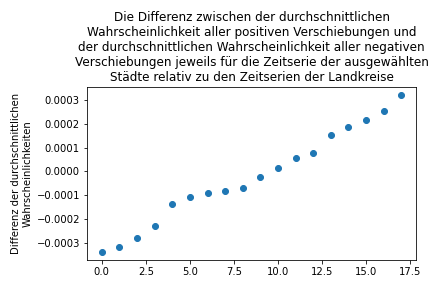
\includegraphics[width=0.95\textwidth]{figures/Ergebnisse/sum_selected_counties.png}
    \caption{Die Tendenzen der Verschiebung aus den Korrelationsanalysen der ausgewählten Städte und Landkreise.}
    \label{fig:sum_selected_counties}
\end{figure}